\section{Implementing rho calculus on modern computers}

\subsection{Processes and names}
The algebra of process states (recapitulated below for convenience) is
directly and succinctly represented by the $\mathsf{Scala}$ code in
the listing below.

\begin{mathpar}
\inferrule* [lab=process] {} {P, Q \bc \pzero \;\bm\; \mathsf{for}(
  y \leftarrow x )P \;\bm\; x\mathsf{!}(Q) \;\bm\;
  \mathsf{*}x \;\bm\; P\mathsf{|}Q } \and \inferrule* [lab=name] {}
            {x, y \bc \mathsf{@}P }
\end{mathpar}

The fact that this compiles and the types are inhabited can be seen as
a mechanical proof that -- despite the strange mutual recursion
between names and processes -- the algebra is not ill-founded. \\
\\

\begin{lstlisting}
trait ProcessStates {
   type Name

   trait ProcessState
   case class Input(
      channel : Name, variable : Name, cont : ProcessState
   ) extends ProcessState
   case class Output(
      channel : Name, payload : ProcessState
   ) extends ProcessState
   case class Composition(
      left : ProcessState, right : ProcessState
   ) extends ProcessState
   case class Deref( name : Name ) extends ProcessState
}

trait Nominals {
   type Process

   trait Nominal
   case class Quote( proc : Process ) extends Nominal
}

object RhoStates extends ProcessStates with Nominals {
   type Process = ProcessState
   type Name = Nominal
   case object Zero extends Process
}
\end{lstlisting}

\begin{remark}
  Note that this implementation makes it possible to easily
  incorporate other kinds of nominals, such as strings, or deBruijn
  indices, or $\mathsf{URI}$s. The code simply makes a wrapper case
  class that extends the Nominal trait. This correspond to the fact
  that because rho is Turing complete we can create process encodings
  of all of the those data types and simply quote them to get those
  types of names. This illustrates one of the key uses of the notion
  of \emph{namespace} in the rho calculus.
\end{remark}

\begin{remark}
  A namespace is simple a collection of names. This can be given
  extensionally, such as listing out the names that are members of a
  set. Or, it can be given intensionally, by providing a rule for
  recognizing when a name is included in a namespace or
  not. Namespaces are incredibly powerful, and this account is the
  first we know about that tames what is otherwise a typically thorny
  and error-prone account found in mainstream languages.
\end{remark}

Next, we illustrate how to turn these process states into execution on
a modern computer.

\subsection{$\mathsf{RSpace}$: a new kind of key-value store}

It turns out that a variant of the $\mathsf{Linda}$ tuple space where
input is not blocking is the critical innovation to an efficient
implementation. Instead of blocking we turn input from a key into the
storage of a continuation at the key. As the astute reader has already
guessed, (the hashes of) channels become keys.

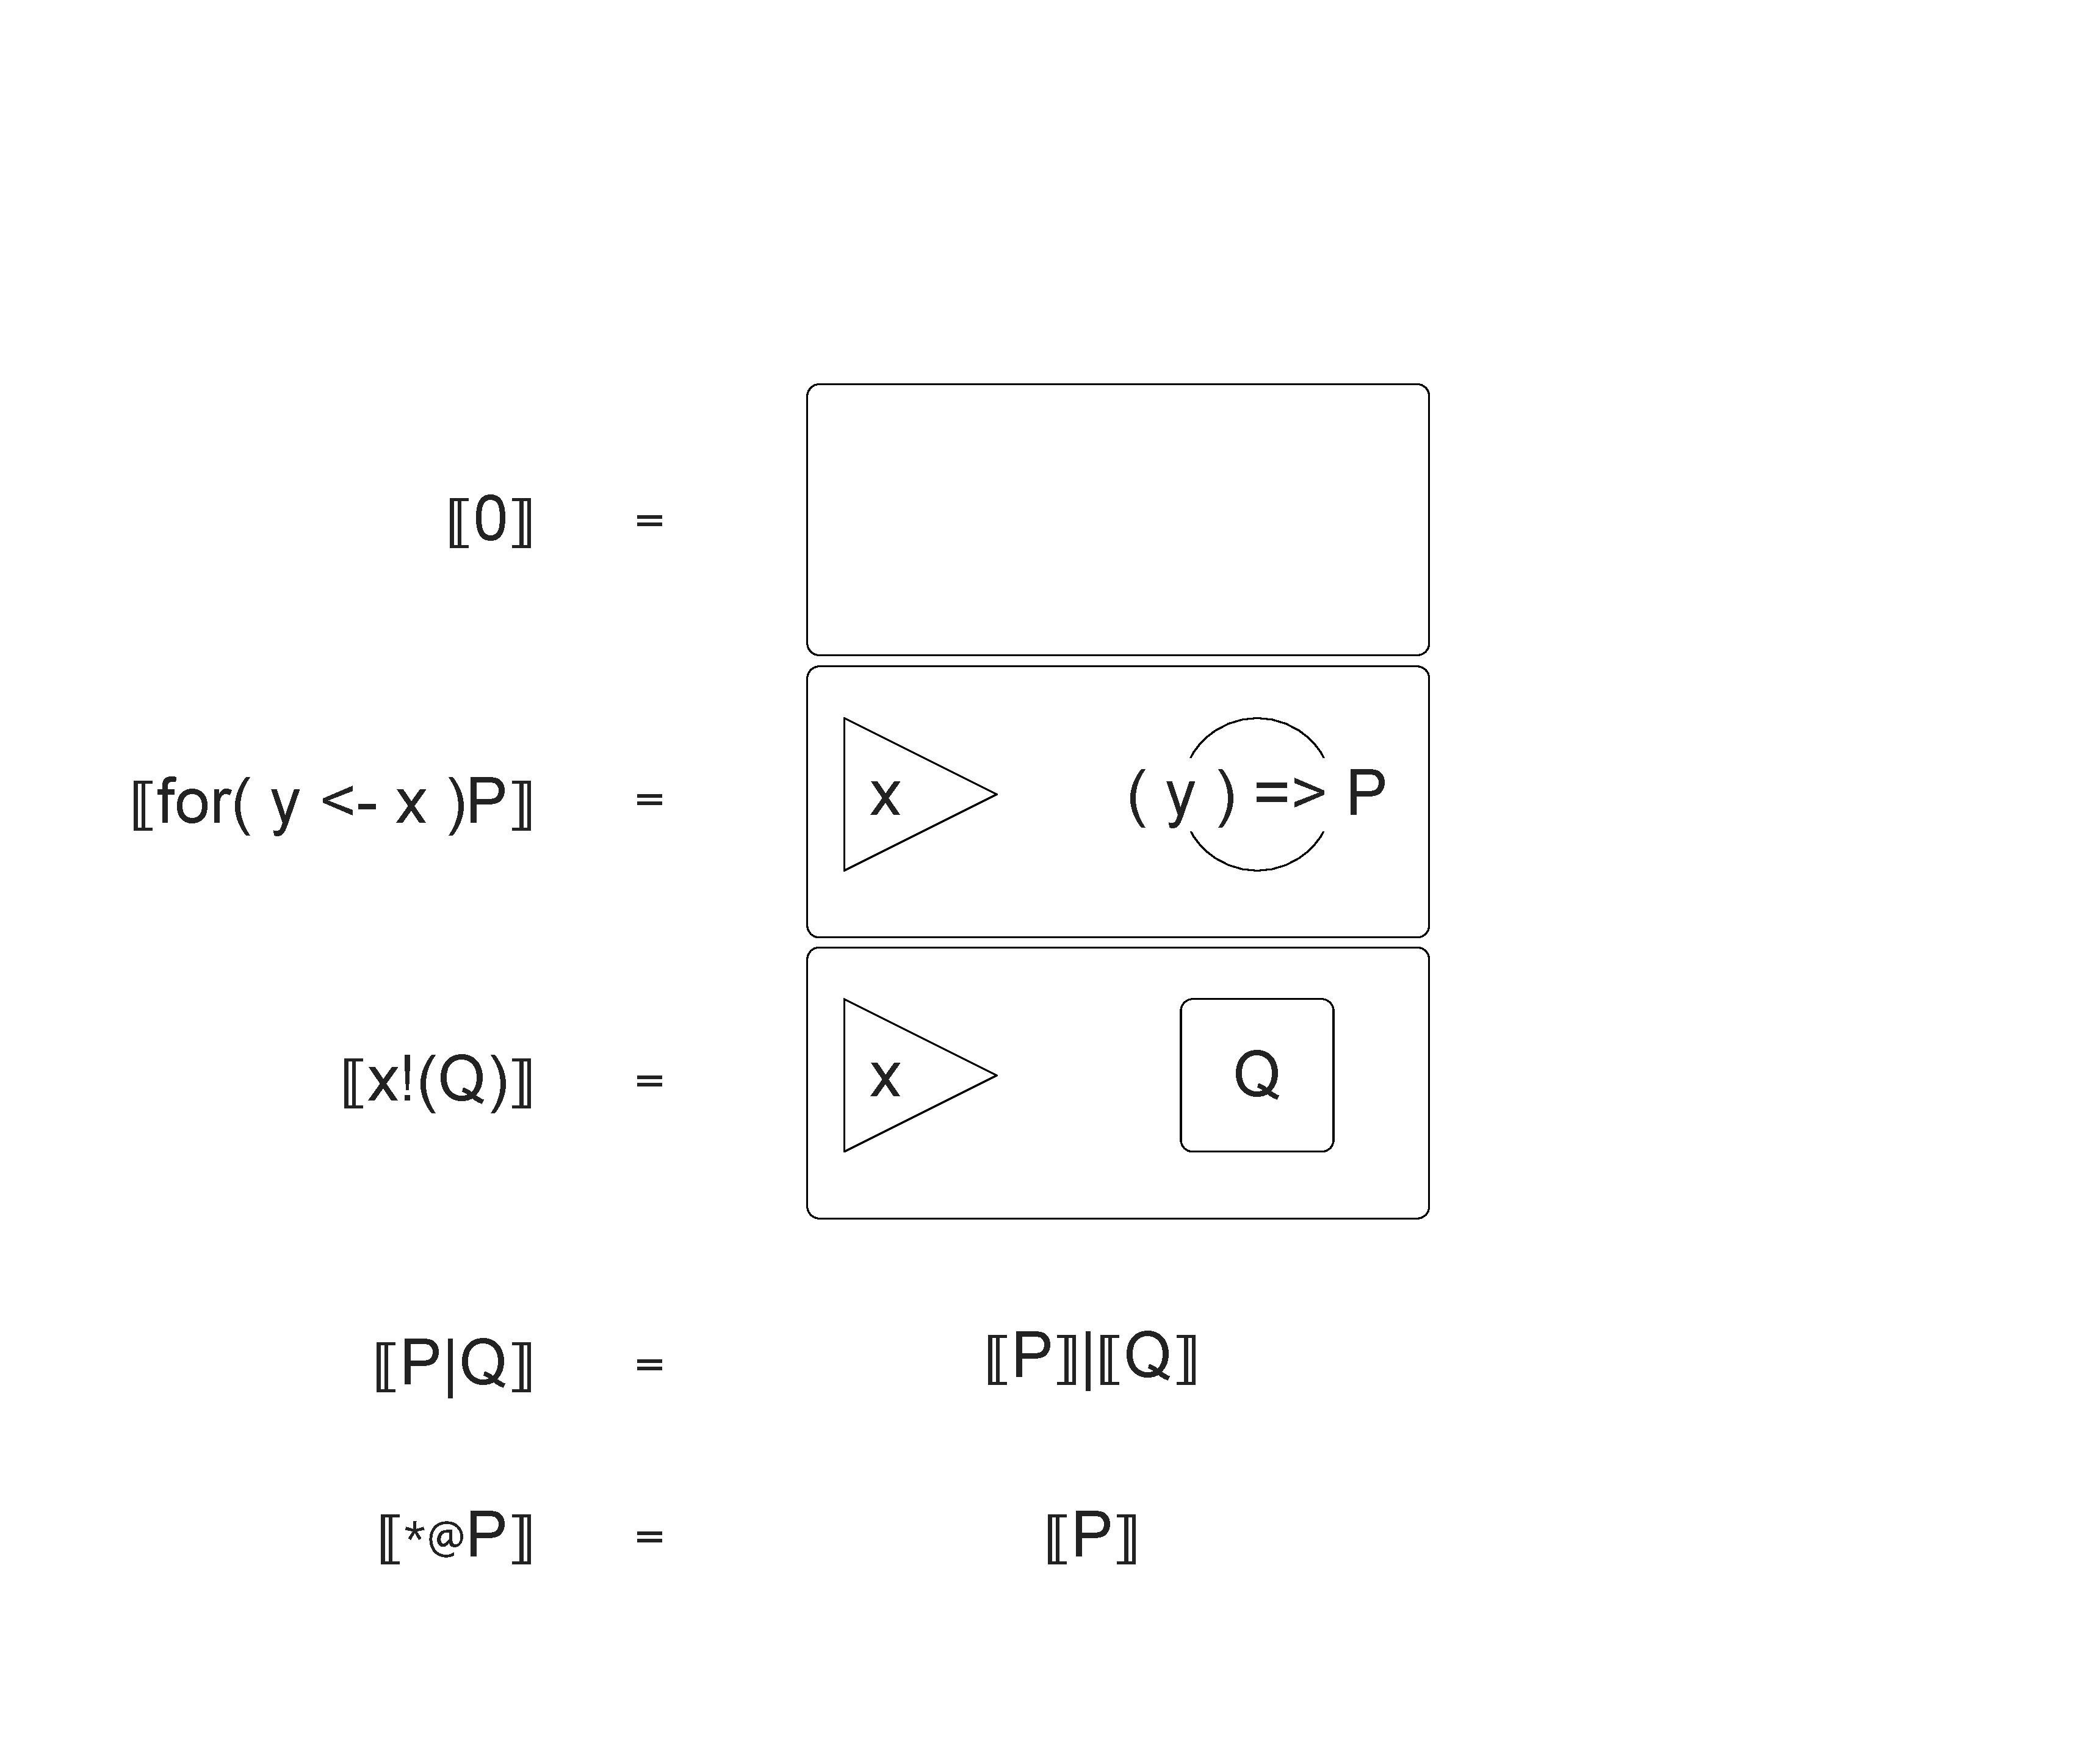
\includegraphics[scale=0.25]{RHO20RSpaceSlide1.pdf} \\

Thus, the diagram above indicates how to turn a given process state
into an $\mathsf{RSpace}$ instance. The 4th equation depends on an
operation on $\mathsf{RSpace}$ instances corresponding to parallel
composition of process states. 

\subsubsection{Parallel composition of $\mathsf{RSpace}s$}
If we are combining two $\mathsf{RSpaces}$ that only have a single
key-value pair, each; and the value is data and not continuation; and
the keys are not equal, then we simply combing them into a single
$\mathsf{RSpace}$ containing both key-value pairs. \\

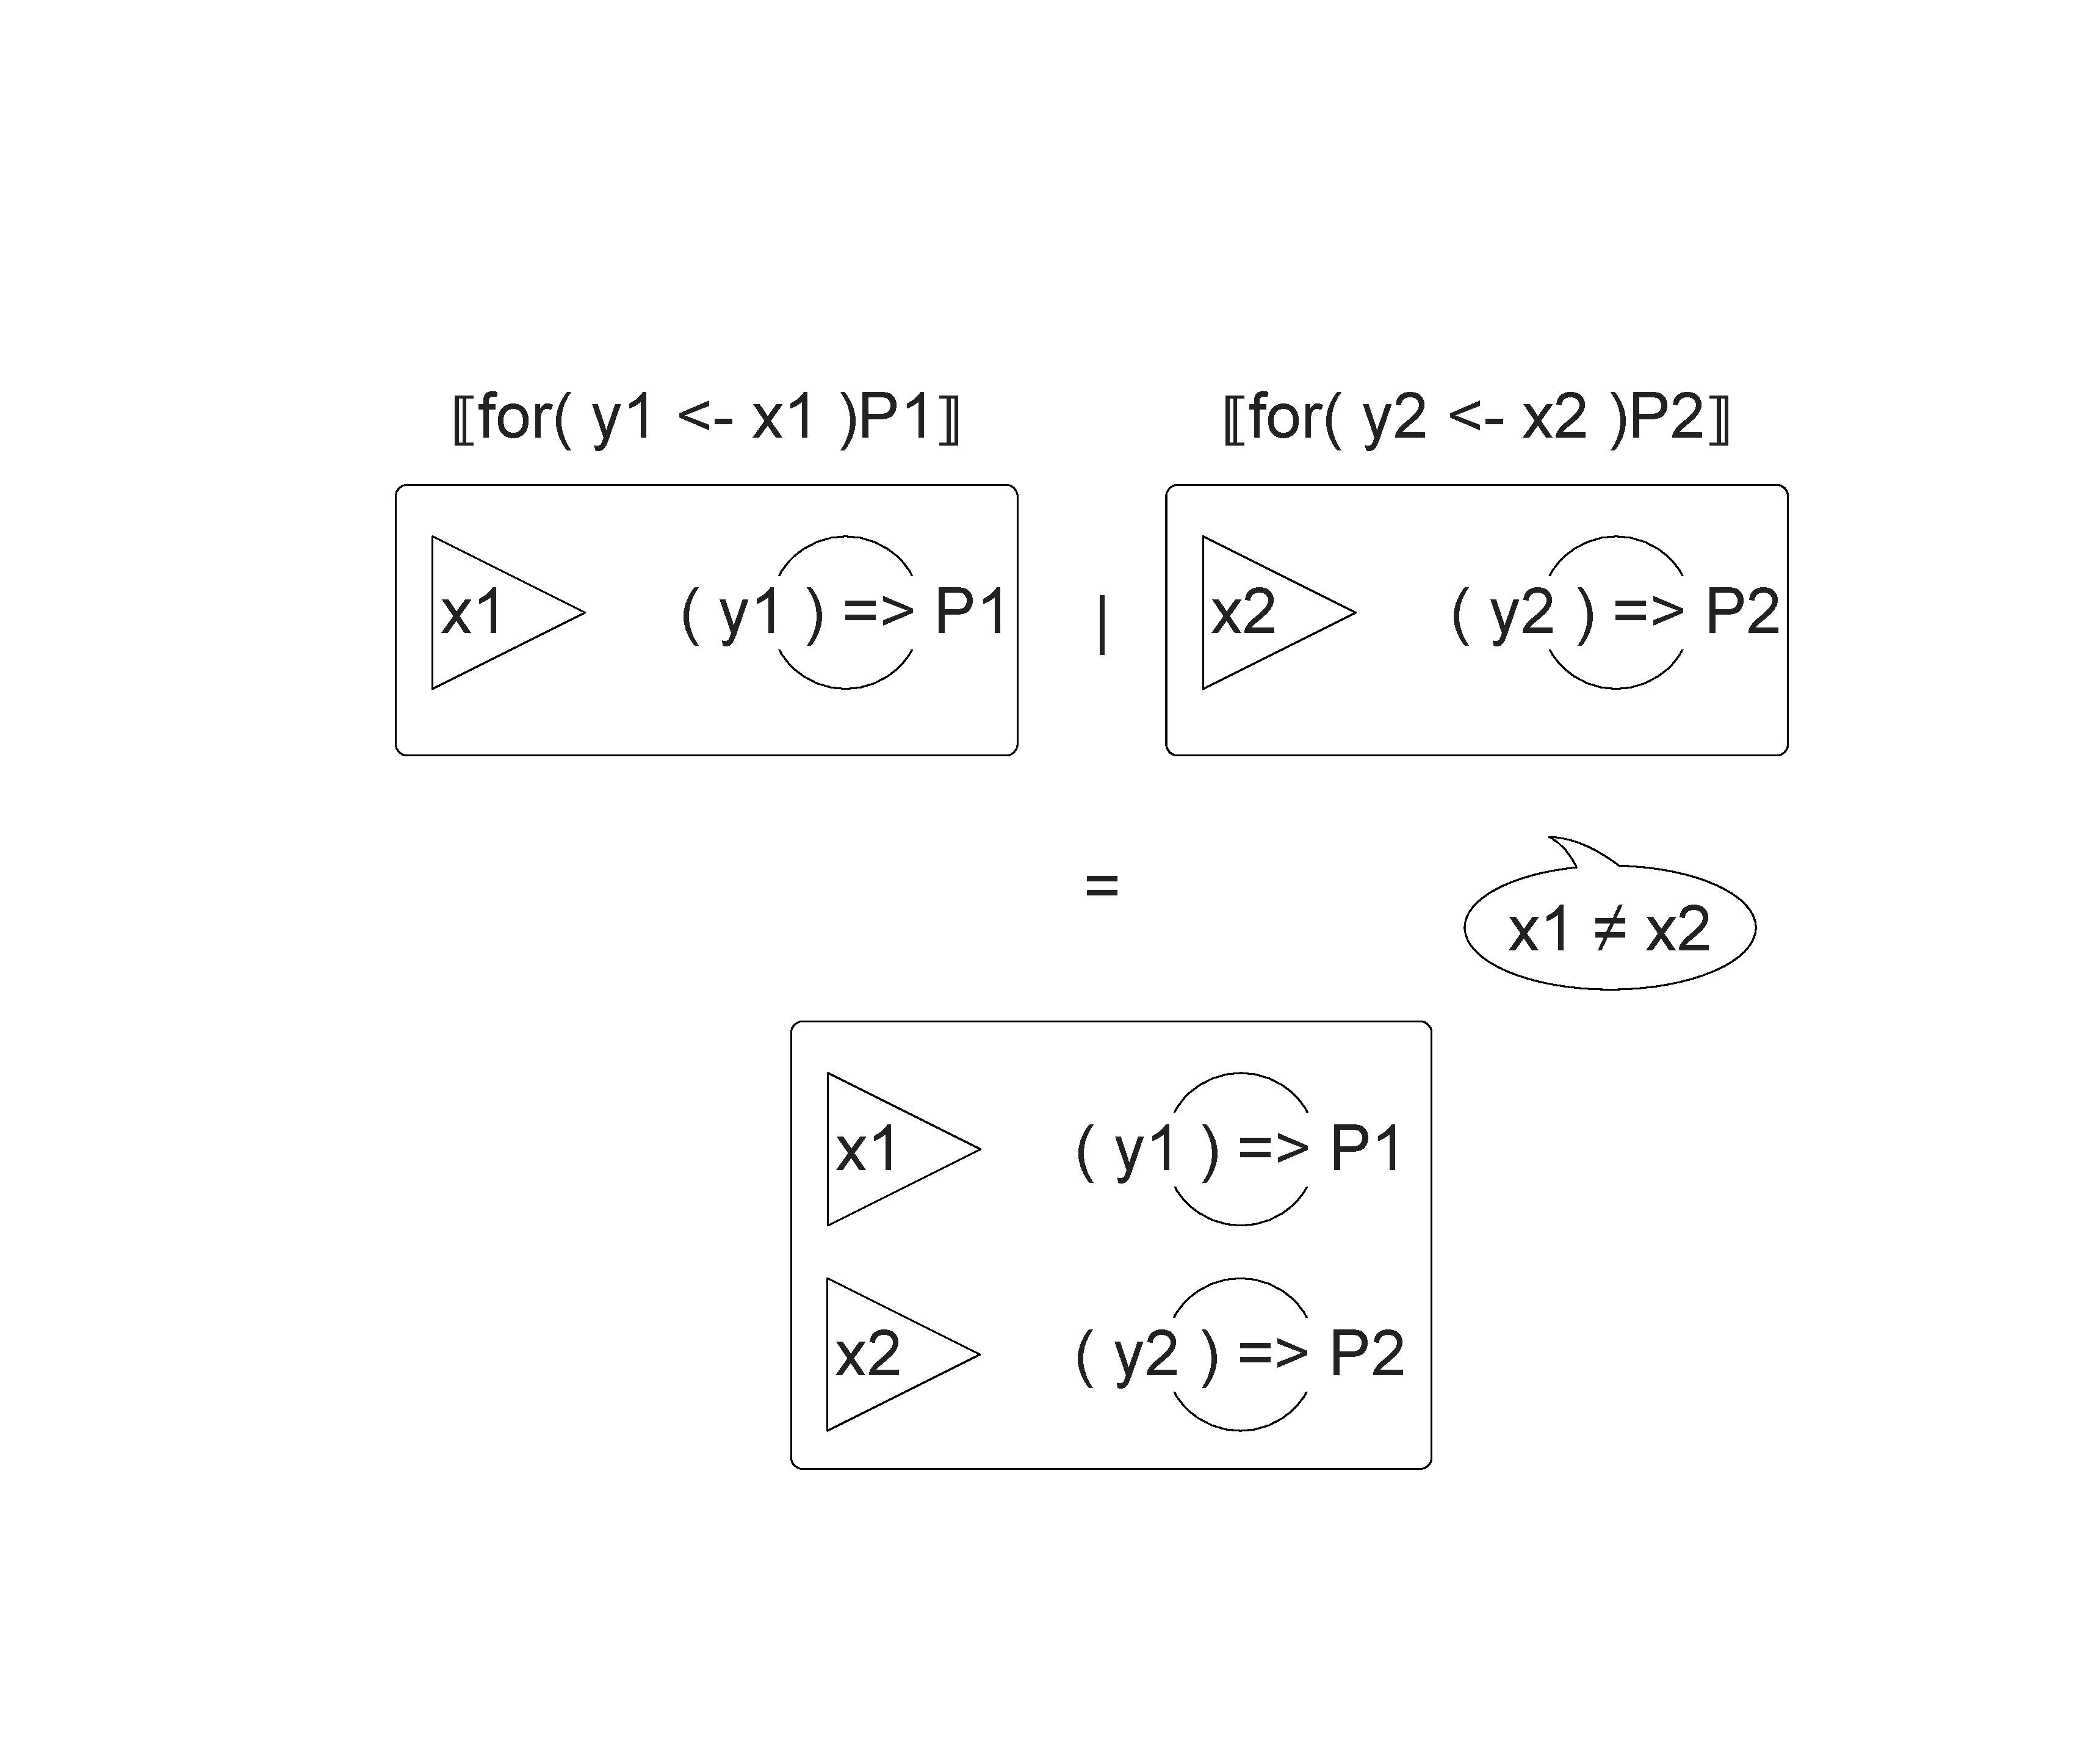
\includegraphics[scale=0.25]{RHO20RSpaceSlide2.pdf}

More generally, if none of the keys of the respective spaces overlaps,
then we simply combine them into a single map. \\

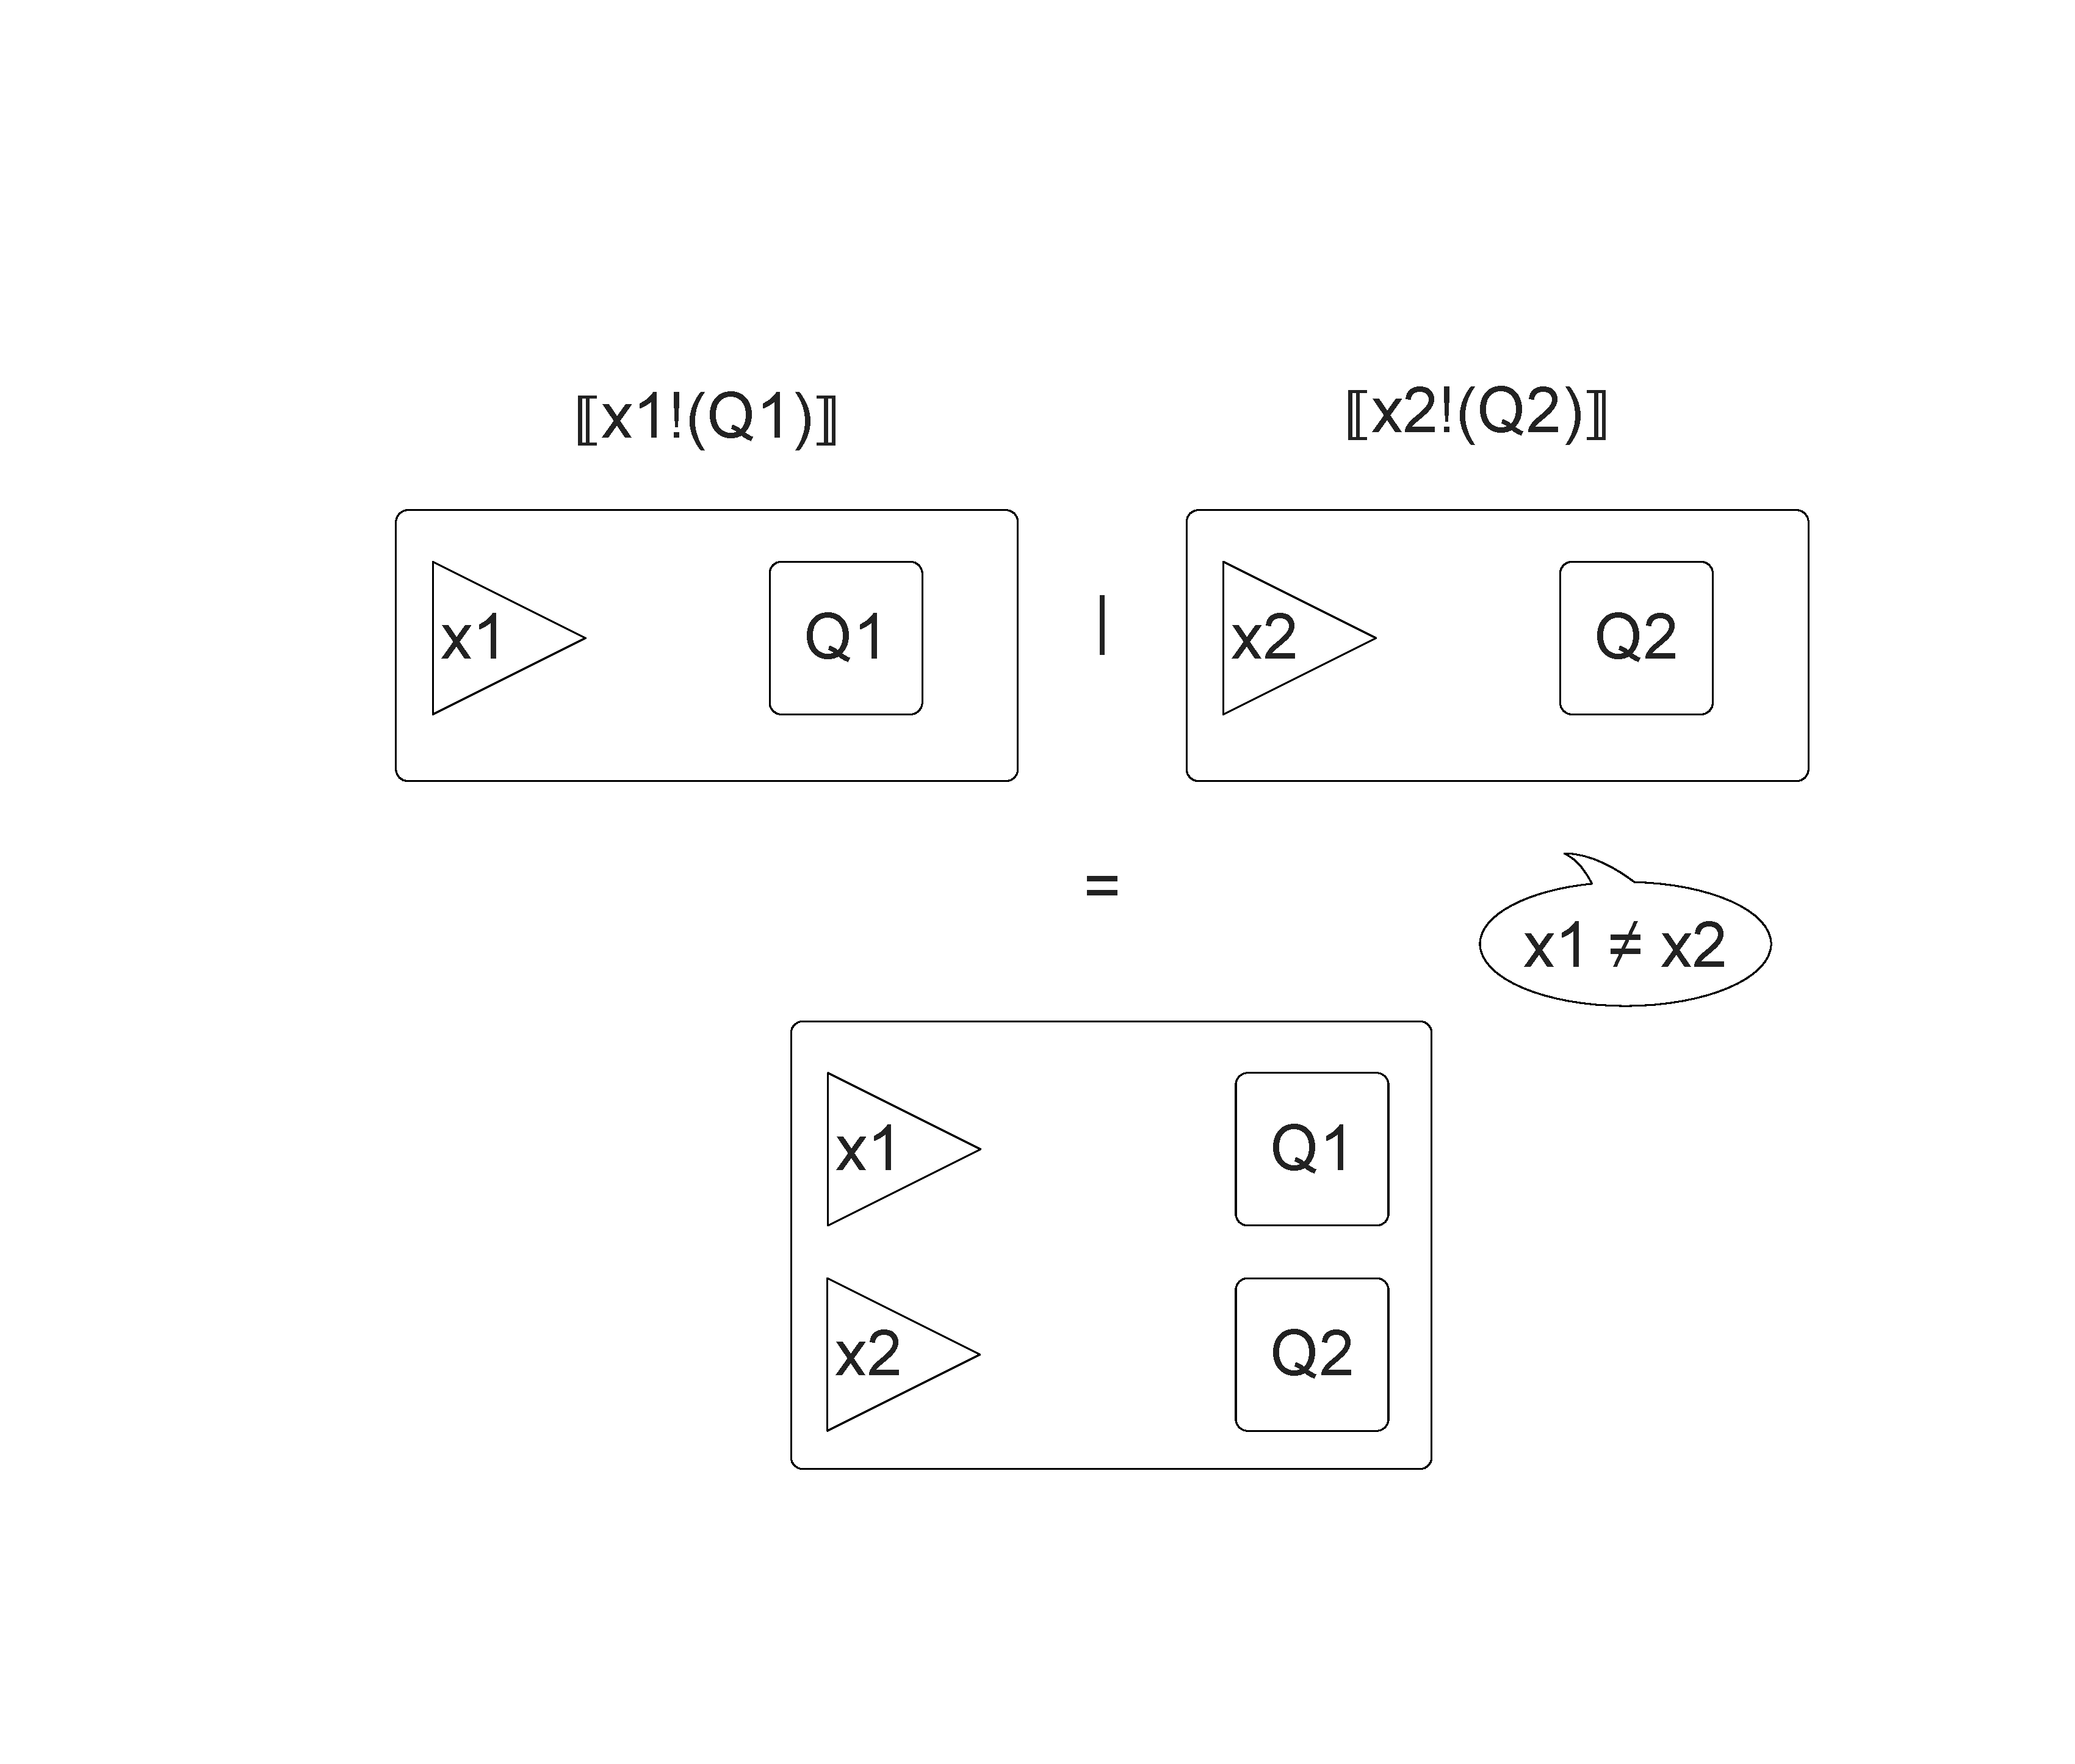
\includegraphics[scale=0.25]{RHO20RSpaceSlide3.pdf}

Similarly, if we are combining two $\mathsf{RSpaces}$ that only have a
single key-value pair, each; and the keys map to continuations; and
the keys are not equal, then we simply combing them into a single
$\mathsf{RSpace}$ containing both key-value pairs. Again, this
generalizes to the case when the the key sets are disjoint.

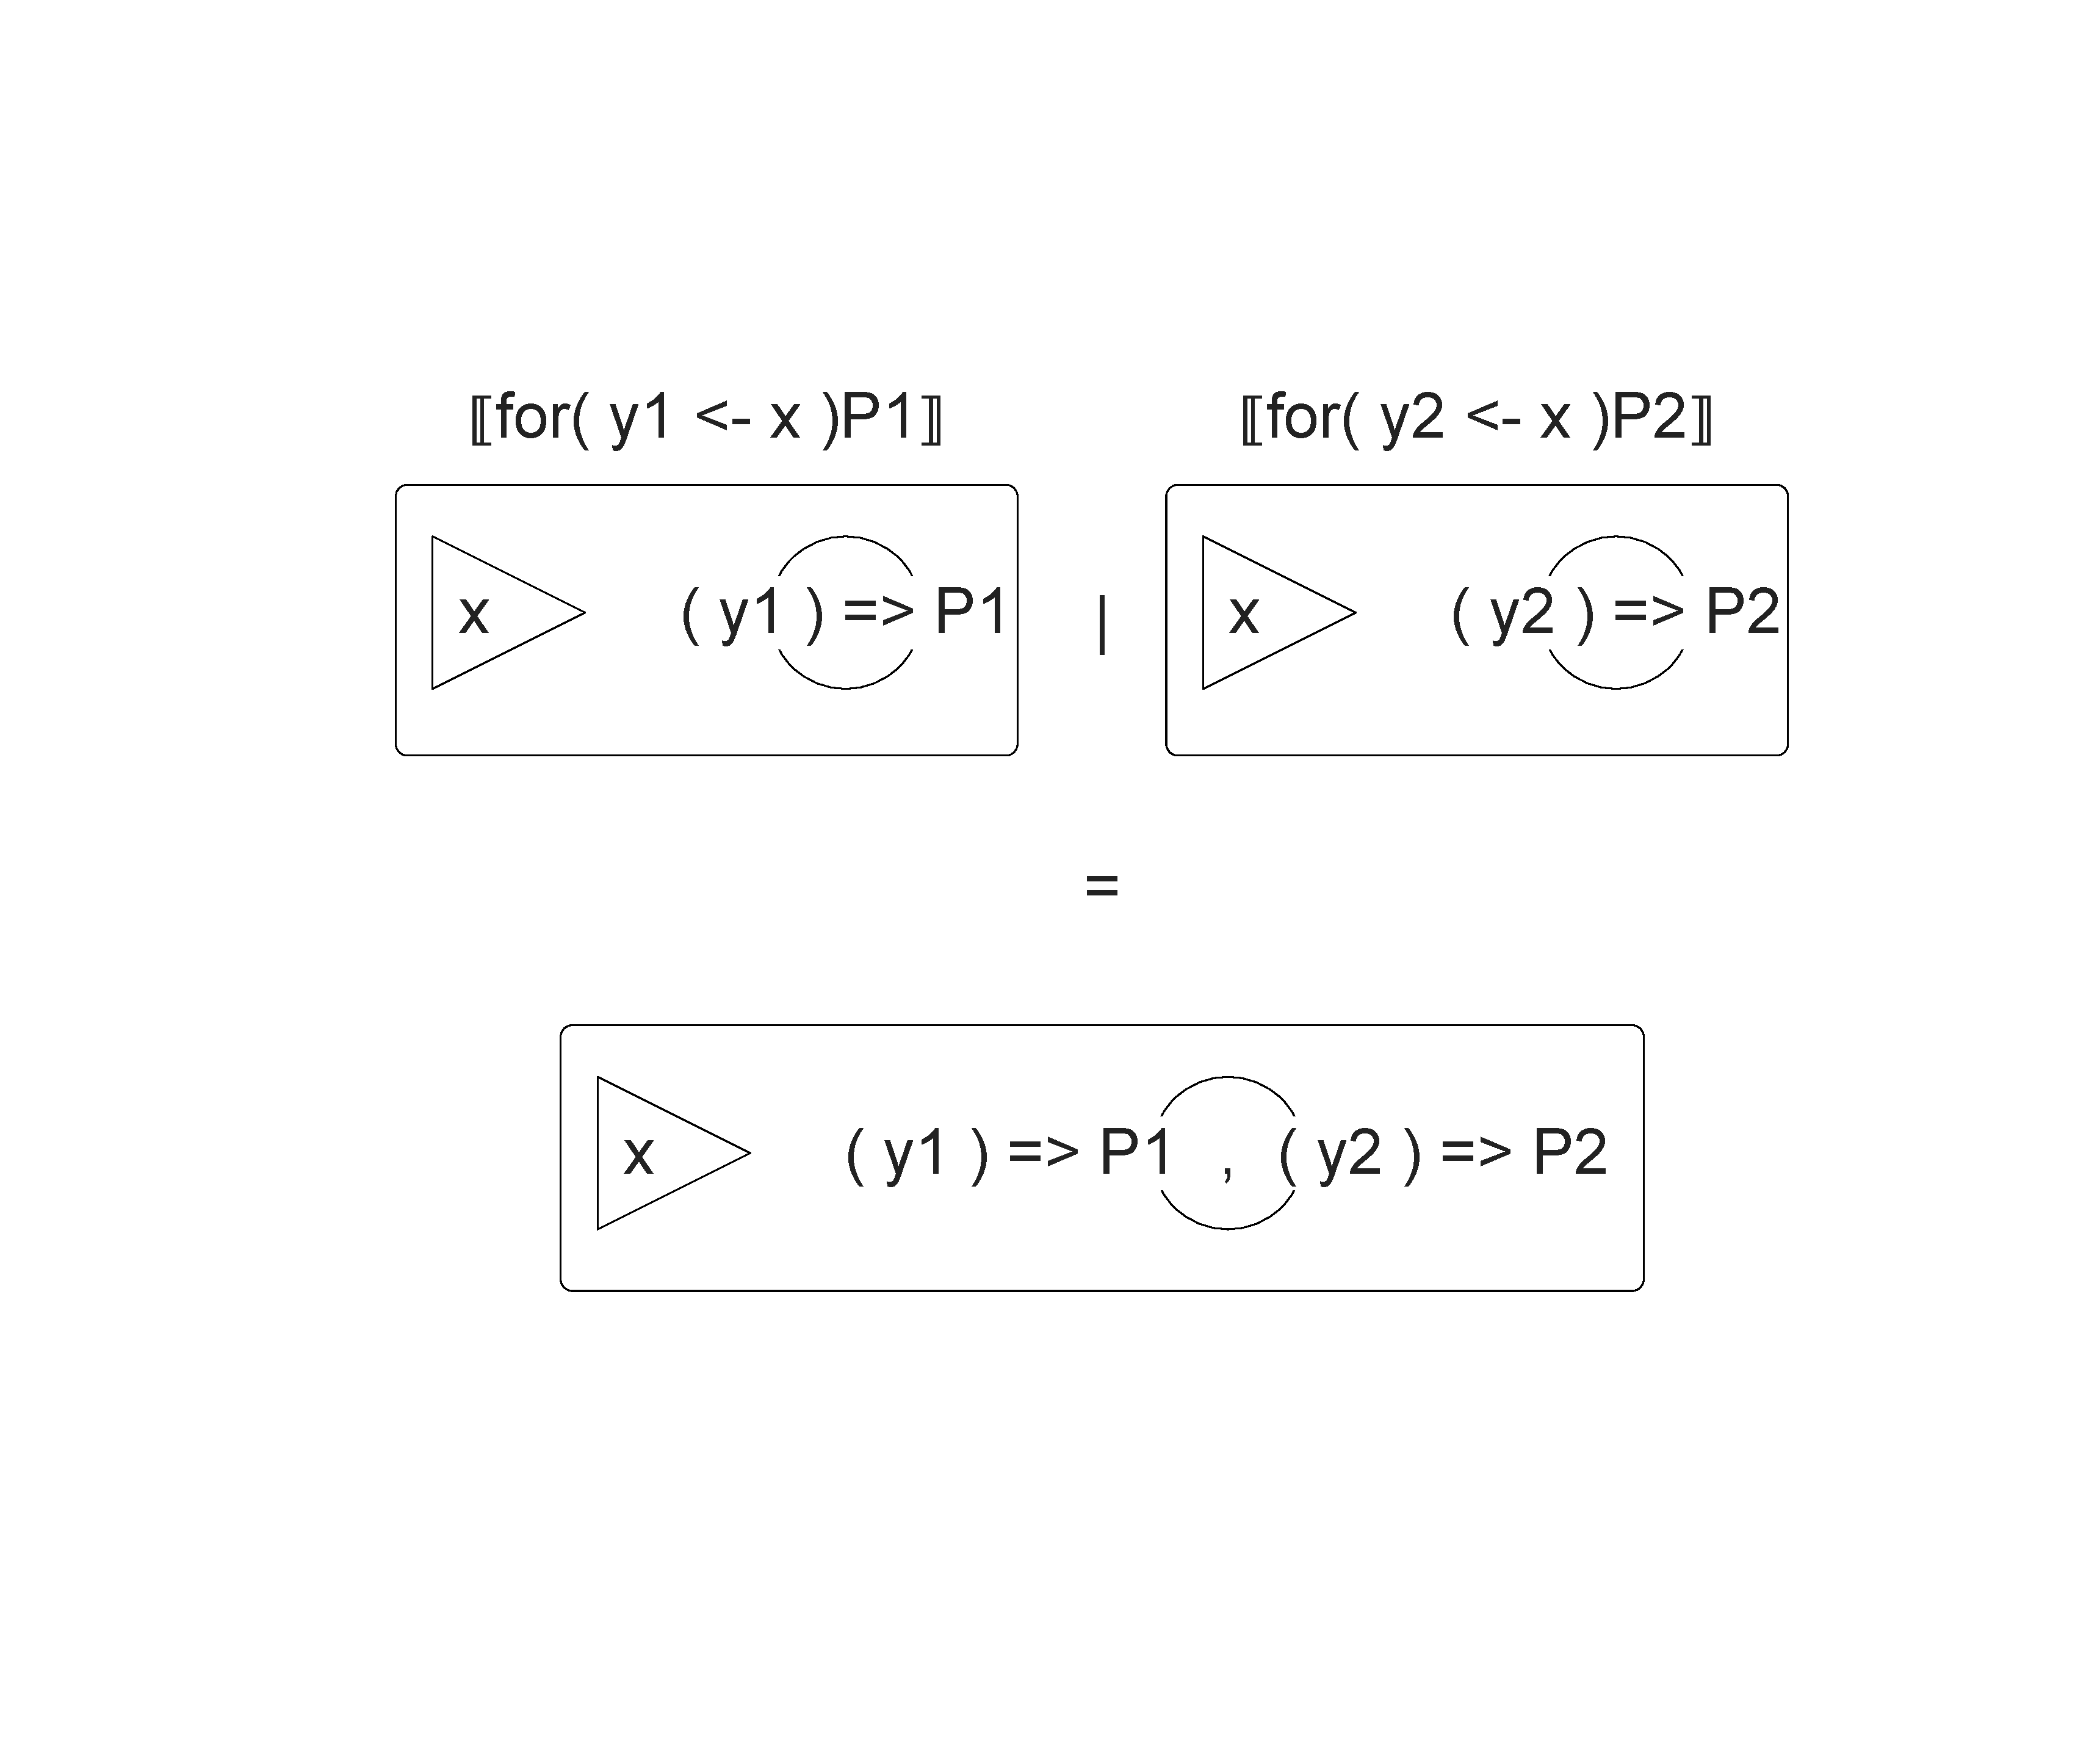
\includegraphics[scale=0.25]{RHO20RSpaceSlide4.pdf}

If we are combining two $\mathsf{RSpaces}$ that only have a single
key-value pair, each; and the keys point to values; and the
keys are equal, then we convert that into a single $\mathsf{RSpace}$
containing where the key maps to a multiset of the values. 

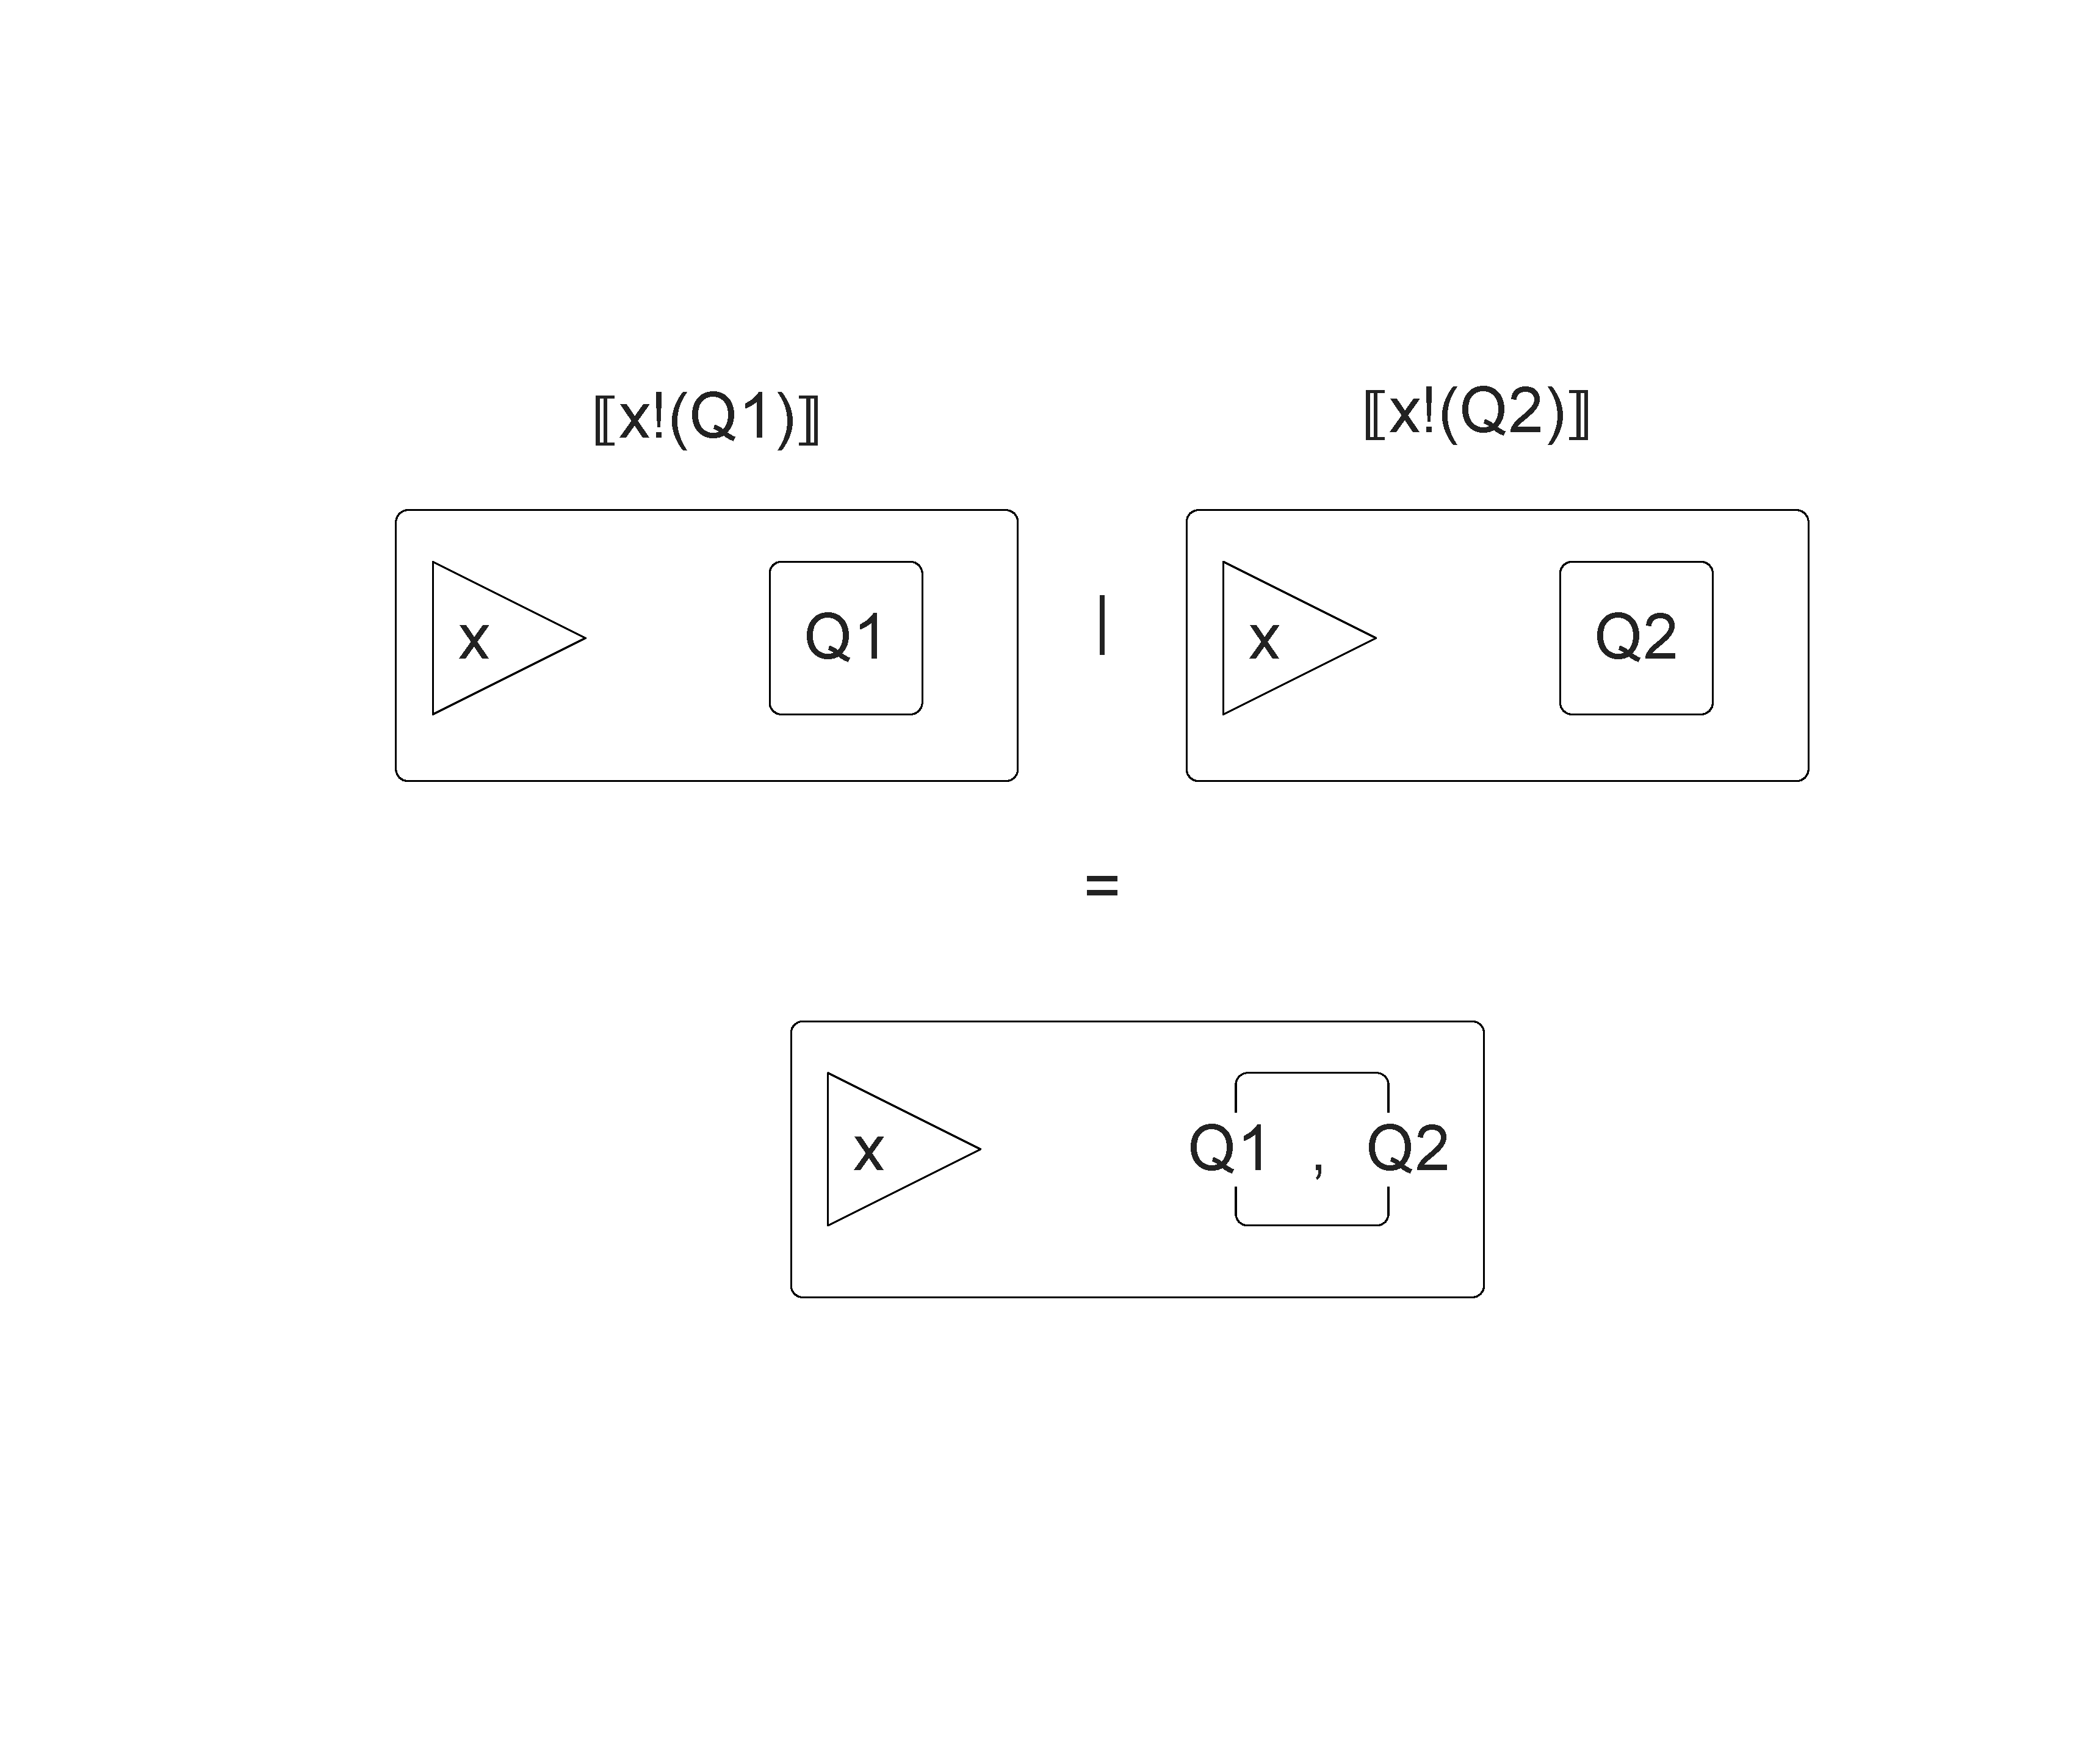
\includegraphics[scale=0.25]{RHO20RSpaceSlide5.pdf}

Dually, for continuations, when we are combining two
$\mathsf{RSpaces}$ that only have a single key-value pair, each; and
the keys point to continuations; and the keys are equal, then we
convert that into a single $\mathsf{RSpace}$ containing where the key
maps to a multiset of the continuations.

These two cases obviously generalize to key sets that are not disjoint
-- but overlapping keys have the same polarity (data versus
continuation) in each space.

What remains is when we have opposite polarity at the same key.

%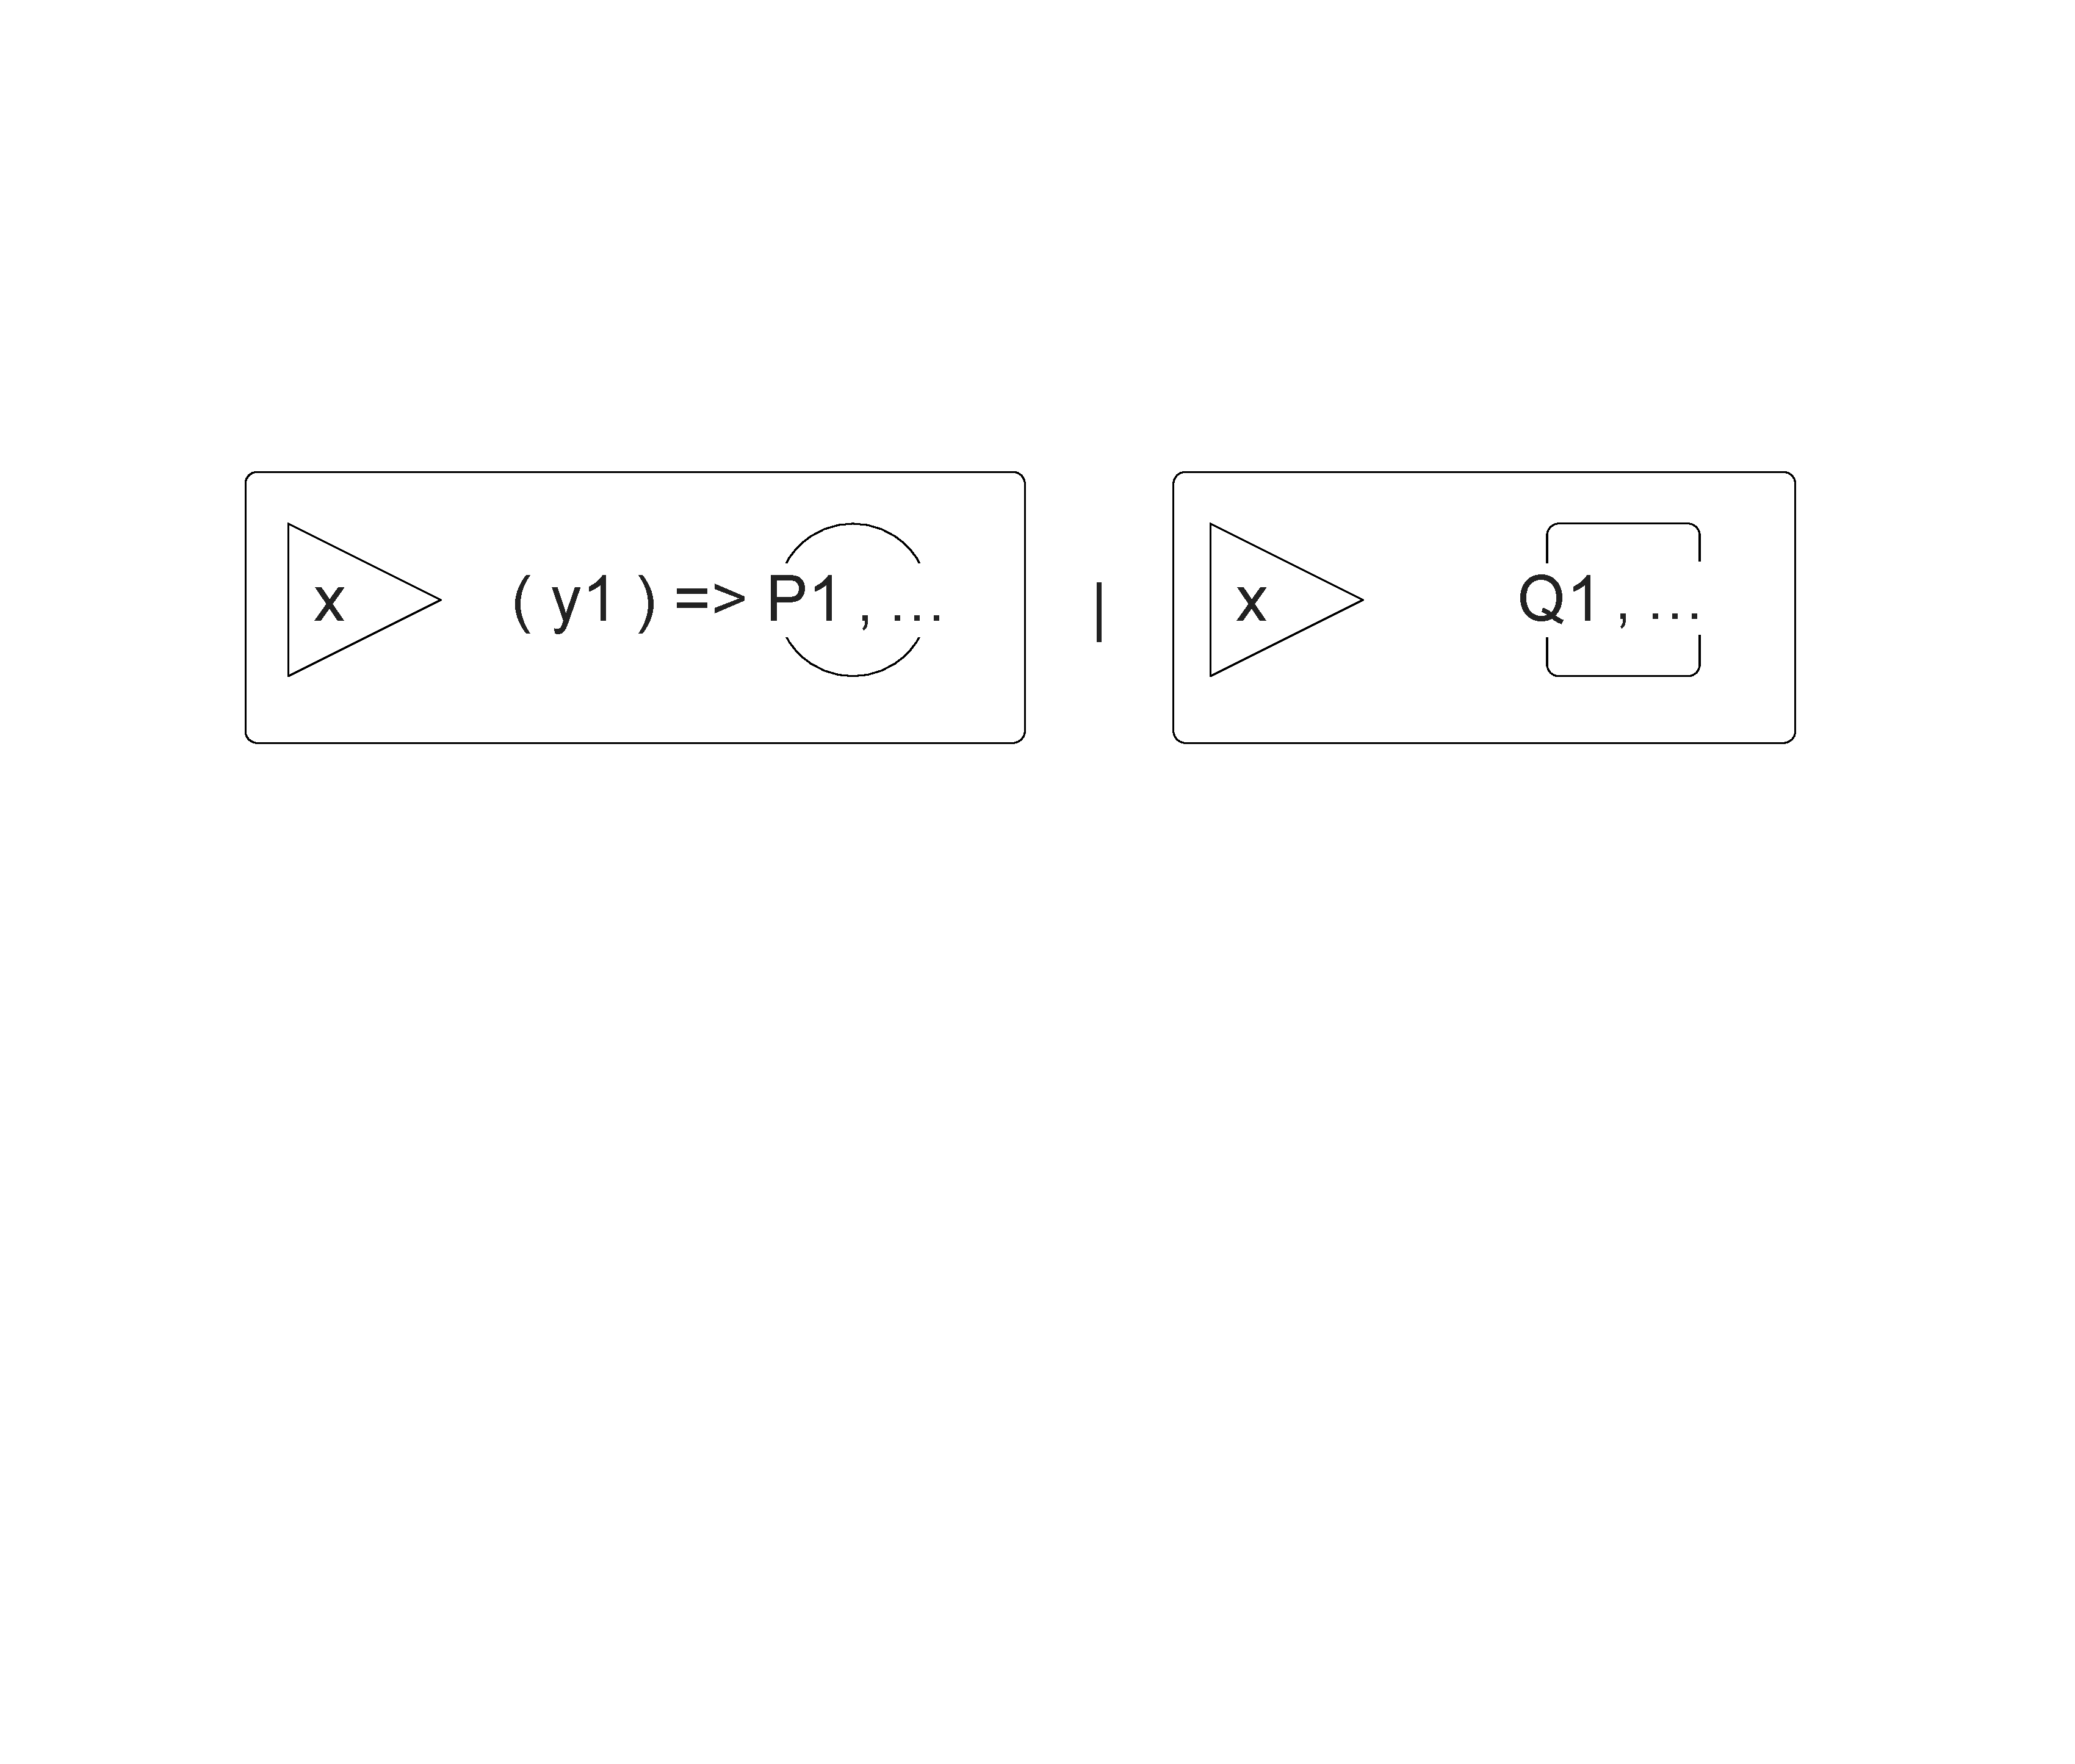
\includegraphics[scale=0.25]{RHO20RSpaceSlide6.pdf}

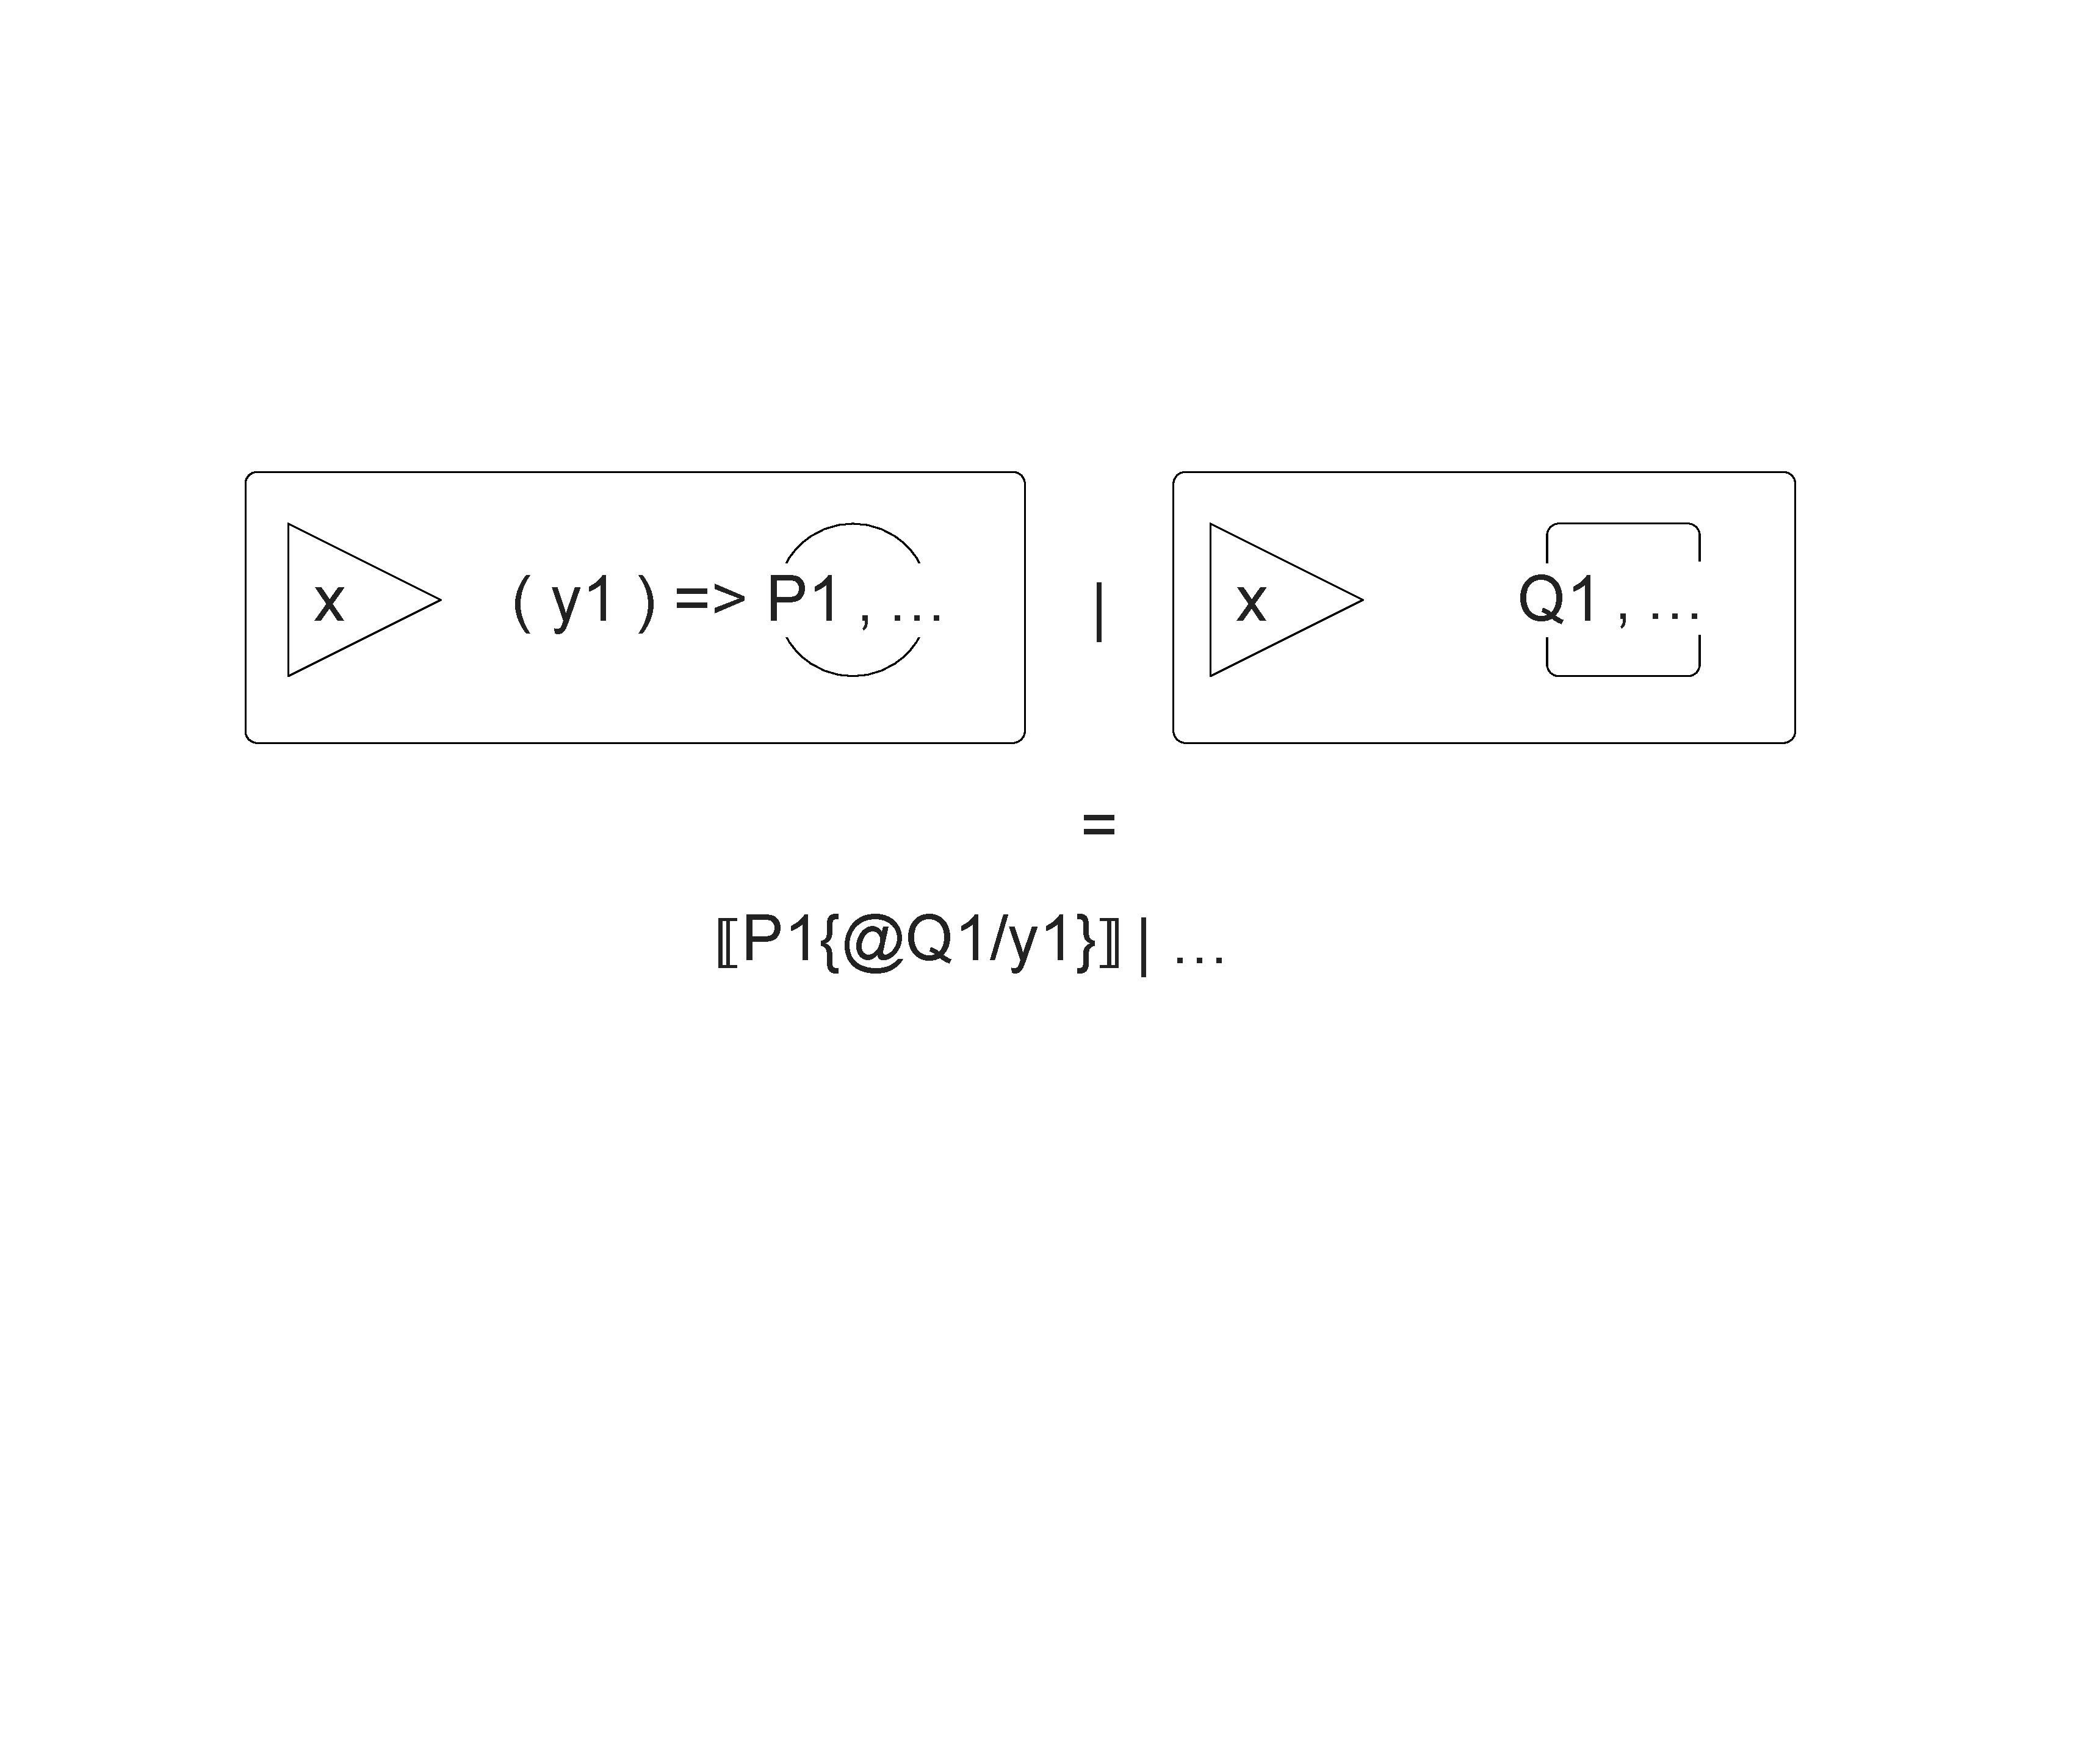
\includegraphics[scale=0.25]{RHO20RSpaceSlide7.pdf}

In this case, one simply zips over the overlapping keys applying the
continuations to the data. \footnote{We leave it to the reader to work
  out the details regarding what happens when the two sets are not the
  same size.}

Note that this is completely sequential execution. The only
non-determinism is the fact that the sets are unordered. Can we do
better? Can we utilize additional physical threads available on modern
hardware to scale execution?

\subsection{Compiling rho to $\mathsf{RSpace}$}

The following code relies on an implementation of $\mathsf{RSpace}$
that supports a polymorphic method $\texttt{p}$ that takes a channel
as its first argument and either a value or a continuation as its
second argument. When it puts a value at a key that maps to a
continuation, it removes the continuation and then applies the
continuation to the value. Dually, when it puts a continuation at a
key that maps to a value it removes the value and applies the
continuation to it. Otherwise, it accumulates values or continuations
in multisets mapped to by keys. Readers interested in more detail can
consult \cite{f1r3fly-io:githubrepo}. \\

\begin{lstlisting}
  trait RhoRuntime {
     def execute( p : RPorQ )( r : RSpace ) : Unit = {
       p match {
         case Zero => { }
         case Input( x, y, p ) => { r.put( x, ( y ) => p ) }
         case Output( x, q ) => { r.put( x, Q ) }
         case Par( p, q ) => {
           val t1 = new Thread() {
             override def run() = { execute( p )( r ) } };
           val t2 = new Thread() {
             override def run() = { execute( q )( r ) }
           }; t1.run(); t2.run()
         }
         case Deref( Ref( p ) ) => { execute( p )( r ) } }
  } }
\end{lstlisting}

\subsubsection{Ordering rho terms}

Another aspect of efficient execution of rho involves ordering
terms. It turns out it is possible to give a total order to rho terms
such that there is a unique representative for each of the equivalence
classes of $\equiv$. Thus, if $\mathsf{N}(P)$ denotes the unique
representative of $[P]_{\equiv}$, then when hashing a channel, say
$\mathsf{@}P$, we calculate actually hash
$\mathsf{@}\mathsf{N}(P)$. Again, for readers interested in more
detail, please see \cite{f1r3fly-io:githubrepo}.

